\documentclass[11pt]{article}
\usepackage{geometry}                
\geometry{letterpaper}                   

\usepackage{graphicx}
\usepackage{amssymb}
\usepackage{epstopdf}
\usepackage{natbib}
\usepackage{amssymb, amsmath}
\DeclareGraphicsRule{.tif}{png}{.png}{`convert #1 `dirname #1`/`basename #1 .tif`.png}

%\title{Title}
%\author{Name 1, Name 2}
%\date{date} 

\begin{document}



\thispagestyle{empty}

\begin{center}
\includegraphics[width=5cm]{ETHlogo.eps}

\bigskip


\bigskip


\bigskip


\LARGE{ 	Lecture with Computer Exercises:\\ }
\LARGE{ Modelling and Simulating Social Systems with MATLAB\\}

\bigskip

\bigskip

\small{Project Report}\\

\bigskip

\bigskip

\bigskip

\bigskip


\begin{tabular}{|c|}
\hline
\\
\textbf{\LARGE{Solving the Travelling Salesman Problem}}\\
\textbf{\LARGE{by Using an Artificial Ant Colony}}\\
\\
\hline
\end{tabular}
\bigskip

\bigskip

\bigskip

\LARGE{Raphaela Wagner \& Giandrin Barandun}



\bigskip

\bigskip

\bigskip

\bigskip

\bigskip

\bigskip

\bigskip

\bigskip

Zurich\\
May 2014\\

\end{center}



\newpage

%%%%%%%%%%%%%%%%%%%%%%%%%%%%%%%%%%%%%%%%%%%%%%%%%

\newpage
\section*{Agreement for free-download}
\bigskip


\bigskip


\large We hereby agree to make our source code for this project freely available for download from the web pages of the SOMS chair. Furthermore, we assure that all source code is written by ourselves and is not violating any copyright restrictions.

\begin{center}

\bigskip


\bigskip


\begin{tabular}{@{}p{3.3cm}@{}p{6cm}@{}@{}p{6cm}@{}}
\begin{minipage}{3cm}

\end{minipage}
&
\begin{minipage}{6cm}
\vspace{2mm} \large Raphaela Wagner

 \vspace{\baselineskip}

\end{minipage}
&
\begin{minipage}{6cm}

\large Giandrin Barandun

\end{minipage}
\end{tabular}


\end{center}
\newpage

%%%%%%%%%%%%%%%%%%%%%%%%%%%%%%%%%%%%%%%



% IMPORTANT
% you MUST include the ETH declaration of originality here; it is available for download on the course website or at http://www.ethz.ch/faculty/exams/plagiarism/index_EN; it can be printed as pdf and should be filled out in handwriting


%%%%%%%%%% Table of content %%%%%%%%%%%%%%%%%

\tableofcontents

\newpage

%%%%%%%%%%%%%%%%%%%%%%%%%%%%%%%%%%%%%%%



\section{Abstract}

\section{Individual contributions}
\subsection{Raphaela Wagner}
With the aim of achieving a good model for solving the travelling salesman problem by the use of artificial ants Raphaela helped the group understanding the underlying paper and the included model. She contributed a great amount of explanations and ideas how to approach the whole project. \\
In a second step she took care of how to implement the raw data from the TSP-library into MATLAB and transform it to a usable form. Further more she coded the functions "eta.m", "global\_pheromene\_update.m", "test\_funktionen.m" and "update.m" and helped improving and correcting the main program. \\
After the code was written she did a lot of testing with different problem sets and compared the solution of the program to known solutions. 

When the group got stuck and did not see a way out of a specific problem she was the one to bring along a hot chocolate and cheer the group up again.

\subsection{Giandrin Barandun}
The paper which is thought to be reconstructed on the following pages was selected and suggested to the group by Giandrin and during the whole process he tried to have some influence on the project with his wide technical understanding of the problem. \\
The codes for the functions "prob\_dist.m", "calc\_Lnn.m", "choose\_city.m", "main\_initialize\_system.m", "coordinates.m" and "calc\_dist.m" are his contributions as well as the collaboration on the main program. He searched the internet for known TS-problems and their solutions and put all data in a readable form. A lion's share for the program working at the end was his bug fixing in all the functions and programs and combining them to the running model.

\section{Introduction and Motivations}
%Introduction and Motivations

Observing crawling ants how they manage to find a shortest path from a food source to their nest arises the question of how to model such a biological phenomena. It is known that the way ants organize their transporting system is based on a secreted chemical called pheromone. While ants move on a track they deposit a certain amount of pheromone. Since real ants prefer choosing lines of a high pheromone concentration, this messenger ensures that ants follow their members on a certain trail.
To illustrate the effect of pheromone on an ant trail consider Figure \ref{fig:ants}. Real ants follow a path between a food source and their nest (Fig. \ref{fig:ants} A). Placing an obstacle on the trail forces the ants to find a way of restoring the interrupted track (Fig. \ref{fig:ants} B). One expects half of the ants to turn right and half of them to turn left. In the beginning both ways around the obstacle are enriched with approximately the same amount of pheromone (Fig. \ref{fig:ants} C). Since ants that have chosen the shortest path need less time to pass by the obstacle the number of ants per time is bigger compared to those who have chosen the longer path. Consequently the shorter path contains a higher concentration of deposited pheromone than the longer one. This follows from the assumption that all ants secrete the same amount of pheromone and move approximately at the same speed. \\
After a certain time more ants prefer the shorter path containing more pheromone until the longer one is completely neglected to circumvent the obstacle (Fig. \ref{fig:ants} D).\\

\begin{SCfigure}[50]
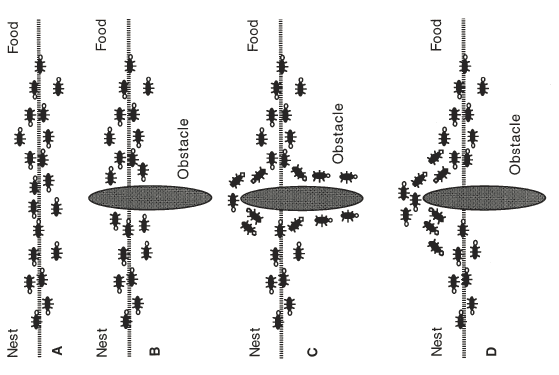
\includegraphics[width=0.4\linewidth]{ants}
\caption{(A): Ants following a trail between food source and their nest. (B): An obstacle is placed to interrupt the track of the ants. (C): The column of ants splits into two groups each choosing a different way to circumvent the obstacle. (D): Due to the higher concentration of pheromone all ants have chosen the shortest path.}
\label{fig:ants}
\end{SCfigure}
\noindent Consulting the literature [1] one finds an interesting paper which uses an ant colony system (ACS) to solve a traveling sales man problem (TSP). Artificial ants, called agents are successively moving on a TSP graph between different cities. In the course of this they are following the constraint to visit each city once and return to their starting point. After all ants have completed their tour, the shortest one is rewarded by increasing the weight of the according tracks. This corresponds to a higher concentration of pheromone on the chosen tour.\\
The goal of this project is to implement the given model (see chapter \ref{sec:model} on page \pageref{sec:model}) from [1] and to calculate the shortest tour for different city environments. Those are obtained from the TSPLIB [2] and correspond to the data used in the reference paper [1]. The aim is to figure out whether our code is able to produce the same length of the shortest tour or not. Next to that, the variation of parameters in the model is analysed. Precisely, these simulations try to answer questions like: How does the shortest tour length depend on the rewarding, i.e. on the amount of pheromone deposited? How fast is the decay in the shortest tour as a function of completed rounds? Moreover, the influence of the number of agents on the time needed to find the shortest tour is investigated.
\section{Description of the Model}
\label{sec:model}
In this model a number of $k$ ants is sent on a network of $m$ cities with every ant starting at the same city. The next ant only starts when the previous ant has finished its tour which means there never are two ants in the network. \\
\subsection{Choosing a City}
Before moving on to the next city an ant has to decide where it wants to go. For this purpose it chooses randomly a number $q$ between zero and one and if this number is smaller or equal than a certain parameter $q_0$ ($q \leqslant q_0$) it looks for the city $s$ which fulfils the following formula:
\begin{equation}
s = \text{arg max}\{[\tau (r,u)] \cdot [\eta (r,u)]^{\beta}\}, \hspace{2cm} u \not\in M_k.
\label{eq:qsmallerq0}
\end{equation}
The current city where the ant stays is denoted by $r$ and only cities can be chosen which are not yet in the ants memory $M_k$ which means the ant has not visited these cities. The matrix $\tau$ stores the information about the amount of pheromone on the edge between city $r$ and city $u$ and the function $\eta$ gives the inverse of the distance between the two cities. \\
If the random number is bigger than $q_0$ ($q > q_0$) the ant randomly chooses one of the remaining unvisited cities and accepts or rejects it according to the probability $p_k$:
\begin{equation}
p_k (r,s) = \frac{[\tau (r,s)] \cdot [\eta (r,s)]^{\beta}}{\sum_{u \not\in M_k}[\tau (r,u)] \cdot [\eta (r,u)]^{\beta}}.
\label{eq:prob}
\end{equation}
This probability basically contains the same formula of $\tau$ and $\eta$ as the one above but is now normalized with the sum over these relations of every unvisited city. One can clearly see that in the beginning the sum is big and the probabilities are small but favouring the edges with more pheromone and lower distance. At the end when only one city is left the sum equals the term in the nominator and the probability becomes one for the last remaining city.
\subsection{Moving Forward and Updating}
Once the city has been chosen the ant moves along the edge and the pheromone on the path is updated according to:
\begin{equation}
\tau (r,s) = (1-\alpha)\cdot \tau(r,s) + \alpha \tau_0.
\label{eq:loctauupdate}
\end{equation}
The newly introduced parameters $\alpha$ and $\tau_0$ are explained in chapter \ref{sec:results}. This update reduces the amount of pheromone on the chosen edge and helps avoiding very strong edges which would be taken by all the ants. \\
At the time the first ant has finished the tour the second one can start while the first ant still keeps in mind the trajectory of its tour which means the sequence of the city it has visited and the length of its tour but deletes its memory such that it is ready for a new tour. When all ants have completed one tour the shortest one is rewarded with pheromone according to the formula:
\begin{equation}
\tau(r,s) = (1-\alpha)\cdot \tau(r,s) + \alpha \Delta \tau(r,s).
\label{eq:globalupdate}
\end{equation}
This update is intended to give the edges along the shortest path a little head start in the following round. With this step the first round is complete and the second round can start.

\subsection{Modifications}

In the above model every ant started at city number 1 and waited for his predecessor to finish his tour completely before it started its own tour. In the paper [1] underlying this report the model was slightly different. All agents are placed randomly on any city in the network and move together. When the first agent chose his second city and moved there he waits until every ant has found its next city. So in every time step all agents move for one city. The difference to the model before is that every ant feels the pheromone on the edges of all the other ants in the network. Whereas in the previous model the second ant only saw the trace the first ant left but did not feel any influence of the still following ants. \\
Another small change which was tested is to increase the award for the shortest path which was found after one round. This means to add a constant amount of pheromone to each edge along the shortest path in the global update formula (equation \ref{eq:globalupdate}).

\begin{equation}
\tau(r,s) = (1-\alpha)\cdot \tau(r,s) + \alpha \Delta \tau(r,s) \textbf{+ 0.1}.
\label{eq:globalupdate2}
\end{equation}

\section{Implementation}
\subsection{Main program}
In the previous section the theoretical understanding of the model was tried to be imparted to the reader. Following in this section is an overview of how the model was implemented in MATLAB. \\
To start with a main program (\textit{main\_initialize\_system.m}) was written which reads the data of a specific TSP and puts it into an upper triangle matrix form which contains the distances between the cities as elements. Further more all parameters like number of rounds and number of contributing ants (agents) can be adjusted in this main program. At the end it activates the function \textit{main\_main.m} with the purpose to find the shortest route. \\
In the main function there are two for-loops, one for the number of rounds and one for the number of ants (agents). For every agent we have a memory of the visited cities (\textit{M\_k})and a trajectory vector which saves the sequence of how the cities where visited. In the first step every ants chooses the next city with help of the function \textit{choose\_city.m} which is described below. The city is added to the memory of the ant and the trajectory vector and the pheromone on the edge is reduced according to the formula on page 75 in the paper. As long as there are unvisited cities this procedure is repeated for the agents and at the end the way to the start city is updated (pheromone, trajectory) and the memory reset. Then the second agent starts his tour. \\
After every agent has finished his route the shortest path is detected and the edges along this route are rewarded with pheromone with help of the trajectory vector and the function \textit{global\_pheromone\_update.m}. At the end of this step the trajectory vector is reset for all ants and the second round can be initialized. After every round the shortest route of the current round is compared to the overall shortest route found until now and then kept or rejected depending on the result of the comparison. \\
When all rounds have been calculated the function gives the shortest path found in any of the rounds.

\subsection{Choose the Next City}


\section{Simulation Results and Discussion}
\label{sec:results}
%Simulation Results and Discussion


\subsection{Length of shortest tour}

In a first attempt the dependency of the shortest tour length on different parameters is analysed. Thereby the number of completed rounds each agent finishes is varied. Moreover the value of the update rate $\alpha$ is optimized and the relative weighting of deposited pheromone and closeness is analysed by changing the parameter $\beta$. \\

The shortest tour length is calculated for a 30 and 51 cities problem (called \emph{oliver30} and \emph{eil51} respectively) and averaged over 10 trials. The distances between the cities are determined using the given coordinates on a two dimensional euclidean plane. The distance $d_\text{i,j}$ between city $i$ and $j$ is then calculated by
\begin{equation}
d = \sqrt((x_i-x_j)^2+(y_i-y_j)^2).
\label{eq:dist}
\end{equation}
For the thirty cities problem \emph{oliver30} the distances are rounded to the next integers. For \emph{eil51} double distances are used.\\

The trajectory vector of the shortest tour is defined as the sequence of city numbers which yields the optimal tour length. For the city environment \emph{oliver30} the solution found in \cite{oli} is given by $[1~3~  4~  5~  6~  7~  8~  9~  10~  11~  12~  13~  14~  15~  16~  17~  18~  19~  20~  21~  22~  23~  25~  24~  26~  27~  28~  29~  30~  2]$. Using equation (\ref{eq:dist}) the total tour length is calculated to $shortest path_\text{solution} = 420$. Comparing it to the sequence obtained from own simulations one observes a slightly different sequence: $[1~2 ~3~  4~  5~  6~  7~  8~  9~  10~  11~  12~  13~  14~  15~  16~  17~  18~  19~  20~  21~  22~  23~  25~  24~  26~  27~  28~  29~  30~  1]$ where the agents don't move from city 30 to 2 but to 1. However, the length of this shortest path also results in $shortest path_\text{simulation}=420$. Obviously, there exist two solution to this symmetric TSP using rounded distances.

In \emph{eil51} the trajectory vector found using the model from \cite{paper} blabalbal. The length is balbalba
$\text{shortest path}_\text{solution} = 426$.

In Figure \ref{fig:roundspeil} and \ref{fig:roundspoli} the dependency of the shortest path length on the number of completed tours is shown. As expected the average length decreases asymptotically towards the value of the optimal path. For both city environments the program achieved to reach the averaged shortest path known from literature \cite{paper} and \cite{oli}. For thirty cities and 400 rounds, $<$shortest path$>$ is in fact equal the best result found, whereas for 51 cities a lot more rounds would have been needed to achieve this. Anyhow, the best result obtained in a single run is $<shortest path>=429.48 \pm 1.86$.\\In Figure \ref{fig:roundspeil} three models have been implemented and tested. The first (white circle dots) correspond exactly to the one described in \cite{paper} where all agents are moving at the same time step. The red squares represent the result obtained by a slightly modified model. The same mathematics has been used but the agents are exploring a new trail one by one. As can be seen, this change has little effect on the value of the shortest tour length and its error.\\ Adapting the pheromone update equations (\ref{eq:localtauupdate}) and (\ref{eq:globalupdate}) on page \pageref{sec:model} by adding a constant of 0.1, results in a steeper fall of the average shortest path. At 2000 rounds the final value does not yet reach the averaged shortest path length from \cite{paper}. One concludes that the added constant was chosen too high such that the global and local update only had a neglecting influence on $\tau(r,s)$.\\




\begin{figure}[h!]
\begin{center}
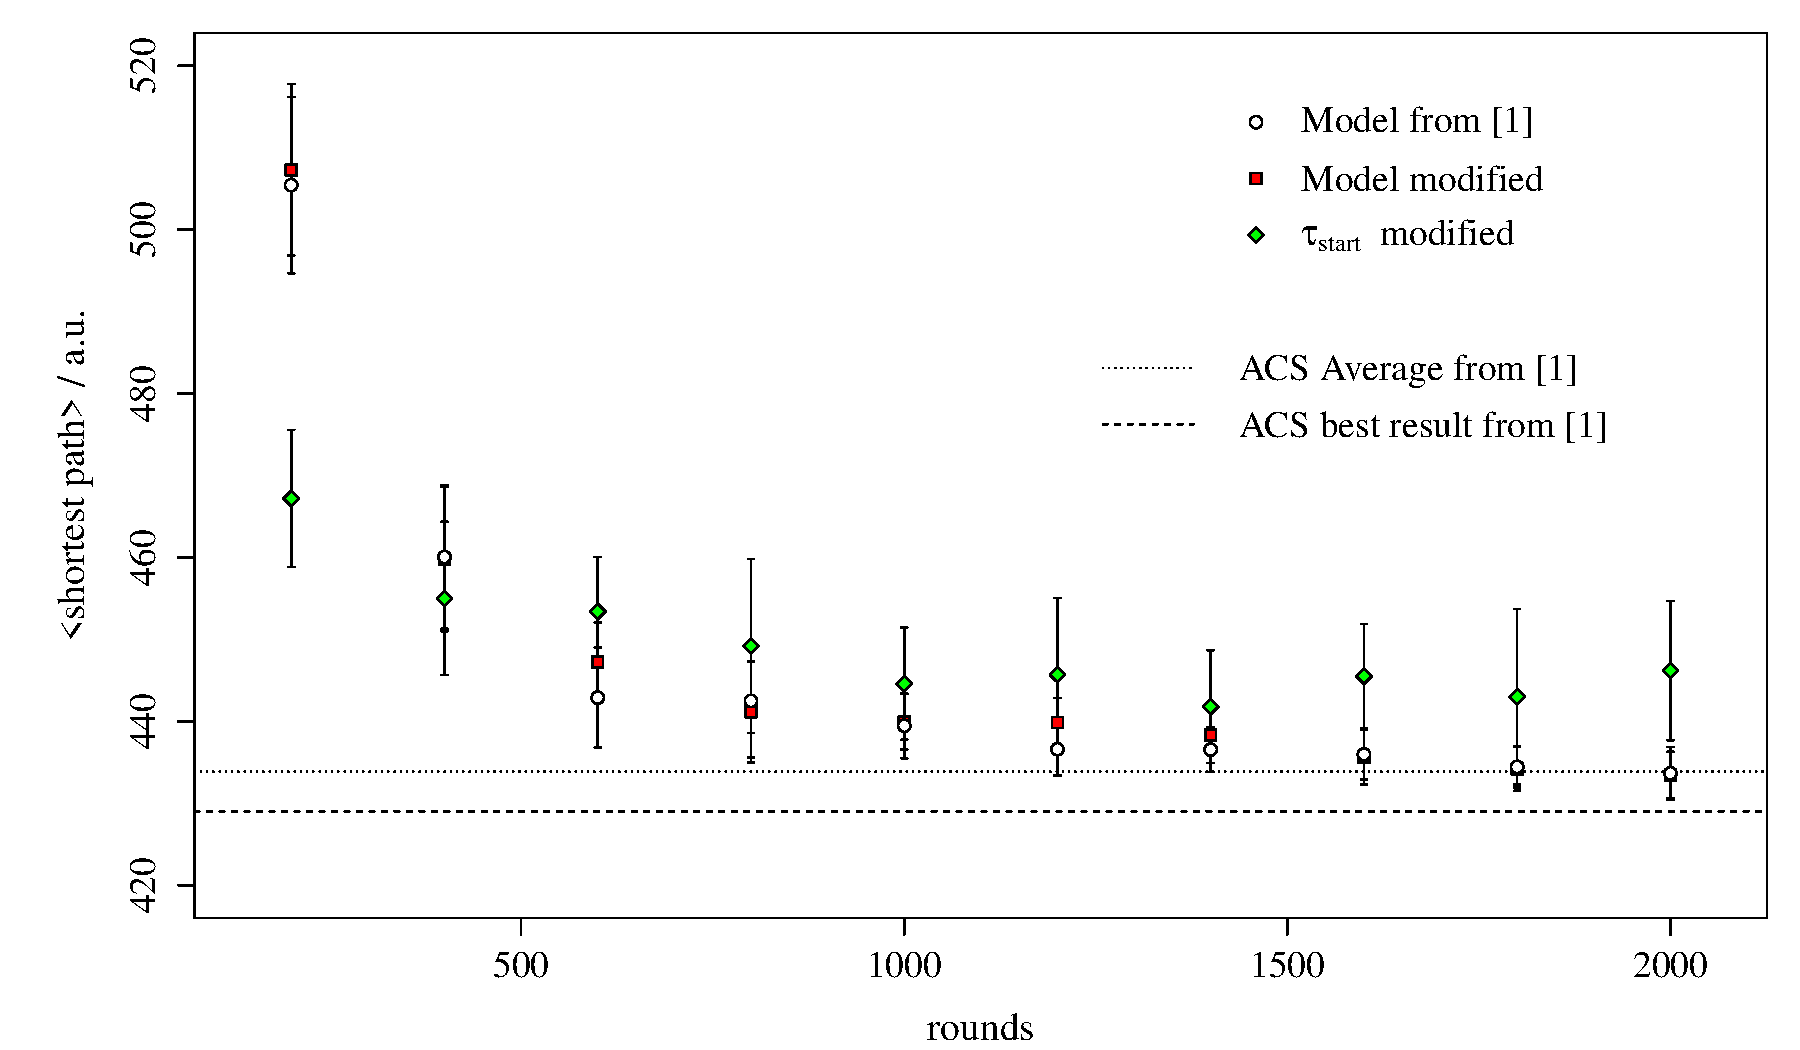
\includegraphics[width=11cm, height= 6 cm]{rounds_vs_shortestpath_eil}
\caption{Shortest tour length averaged over 10 runs for different numbers of rounds. The value approximates the optimal solution for $\approx$ 1200 rounds.}
\label{fig:roundspeil}
\end{center}
\end{figure}


\begin{figure}[h!]
\begin{center}
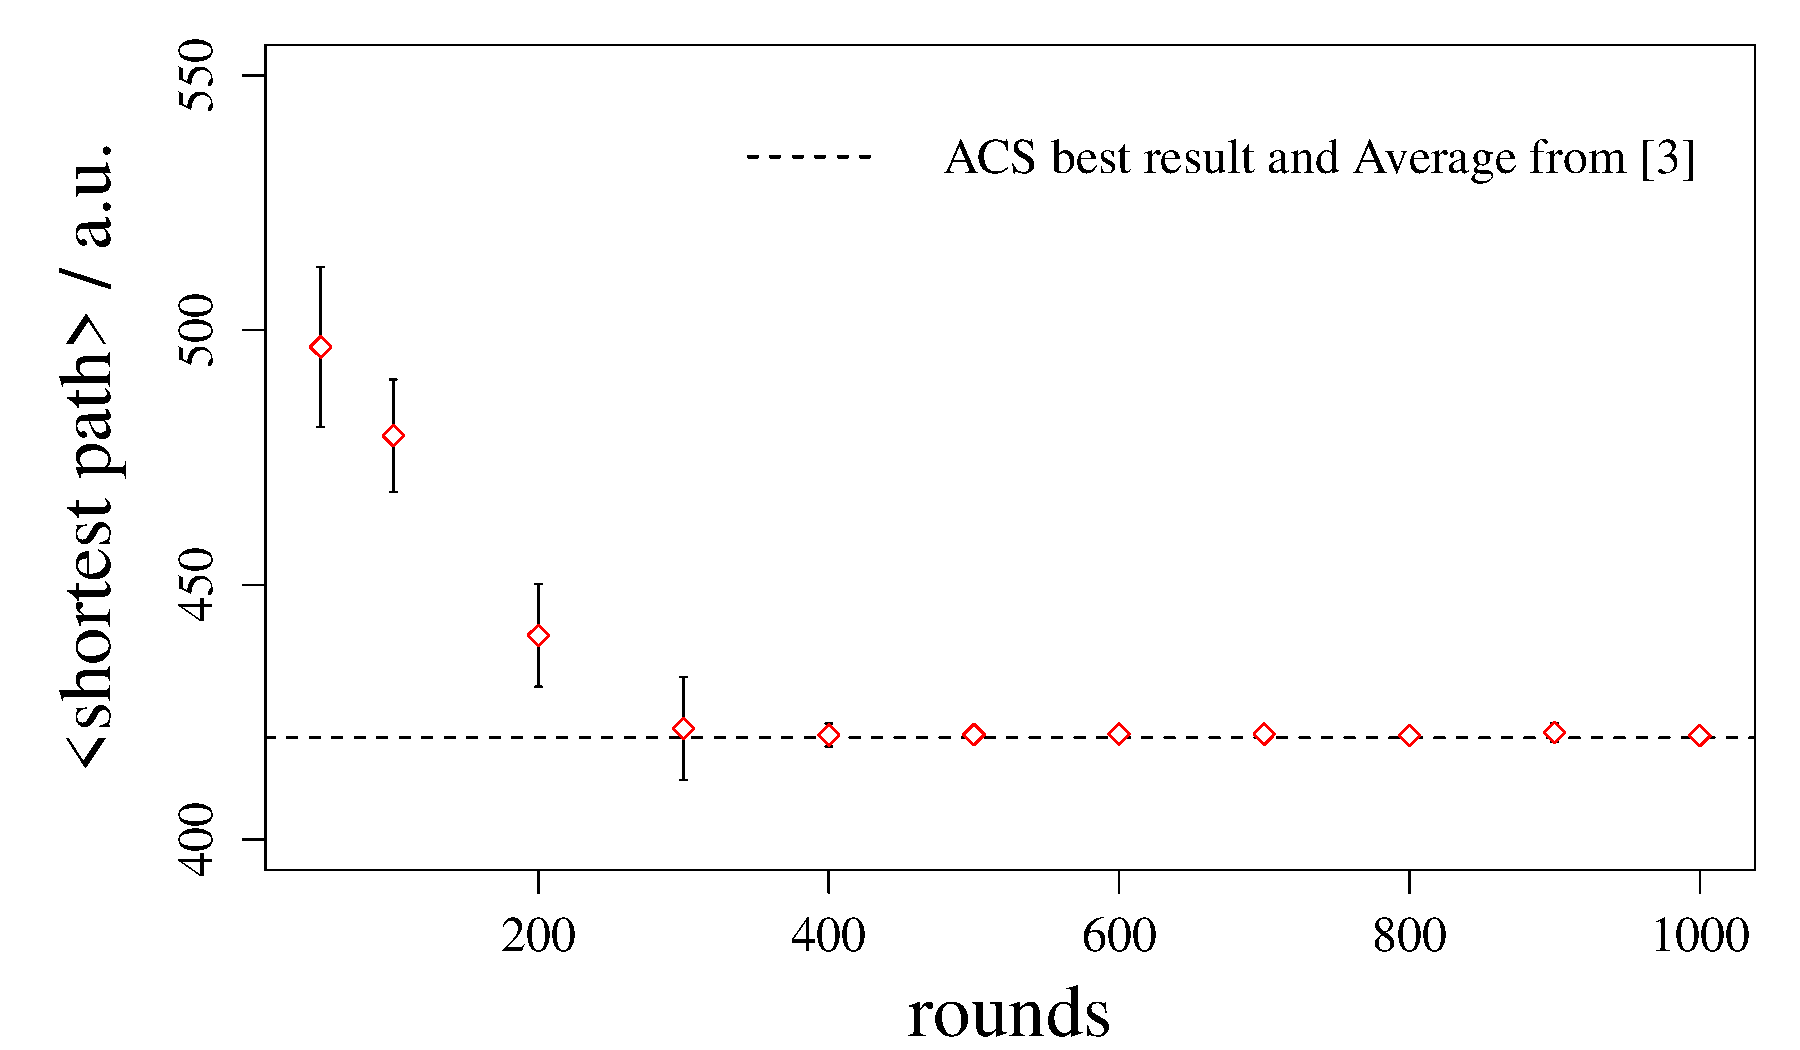
\includegraphics[width=11cm, height= 6 cm]{rounds_vs_shortestpath_oli}
\caption{Shortest tour length averaged over 10 runs for different numbers of rounds. The value approximates the optimal solution for $\approx$ 400 rounds.}
\label{fig:roundspoli}
\end{center}
\end{figure}


Figure \ref{fig:alphasp} illustrates that the averaged shortest path length is optimized for $\alpha$ between 0.1 and 0.3. This is the region where the length of the tour and also the error of the shortest path is minimized. The reason why the shortest path is highest close zero and one, can be understood considering the pheromone update formulas (\ref{eq:localtauupdate}) and (\ref{eq:globalupdate}) on page \pageref{sec:model}. For $\alpha=0$ the local and global pheromone concentration stays constant, no update is made. Hence the cities are only favored by closeness and not by the pheromone concentration anymore. On the other hand, if $\alpha$ is close to one the amount of pheromone after the local update has changed a lot. Randomly chosen trails which deviate from the shortest path will be weighted too much. Therefore the optimal update rate $\alpha$ is expected to be closer to zero. 

\begin{figure}[h!]
\begin{center}
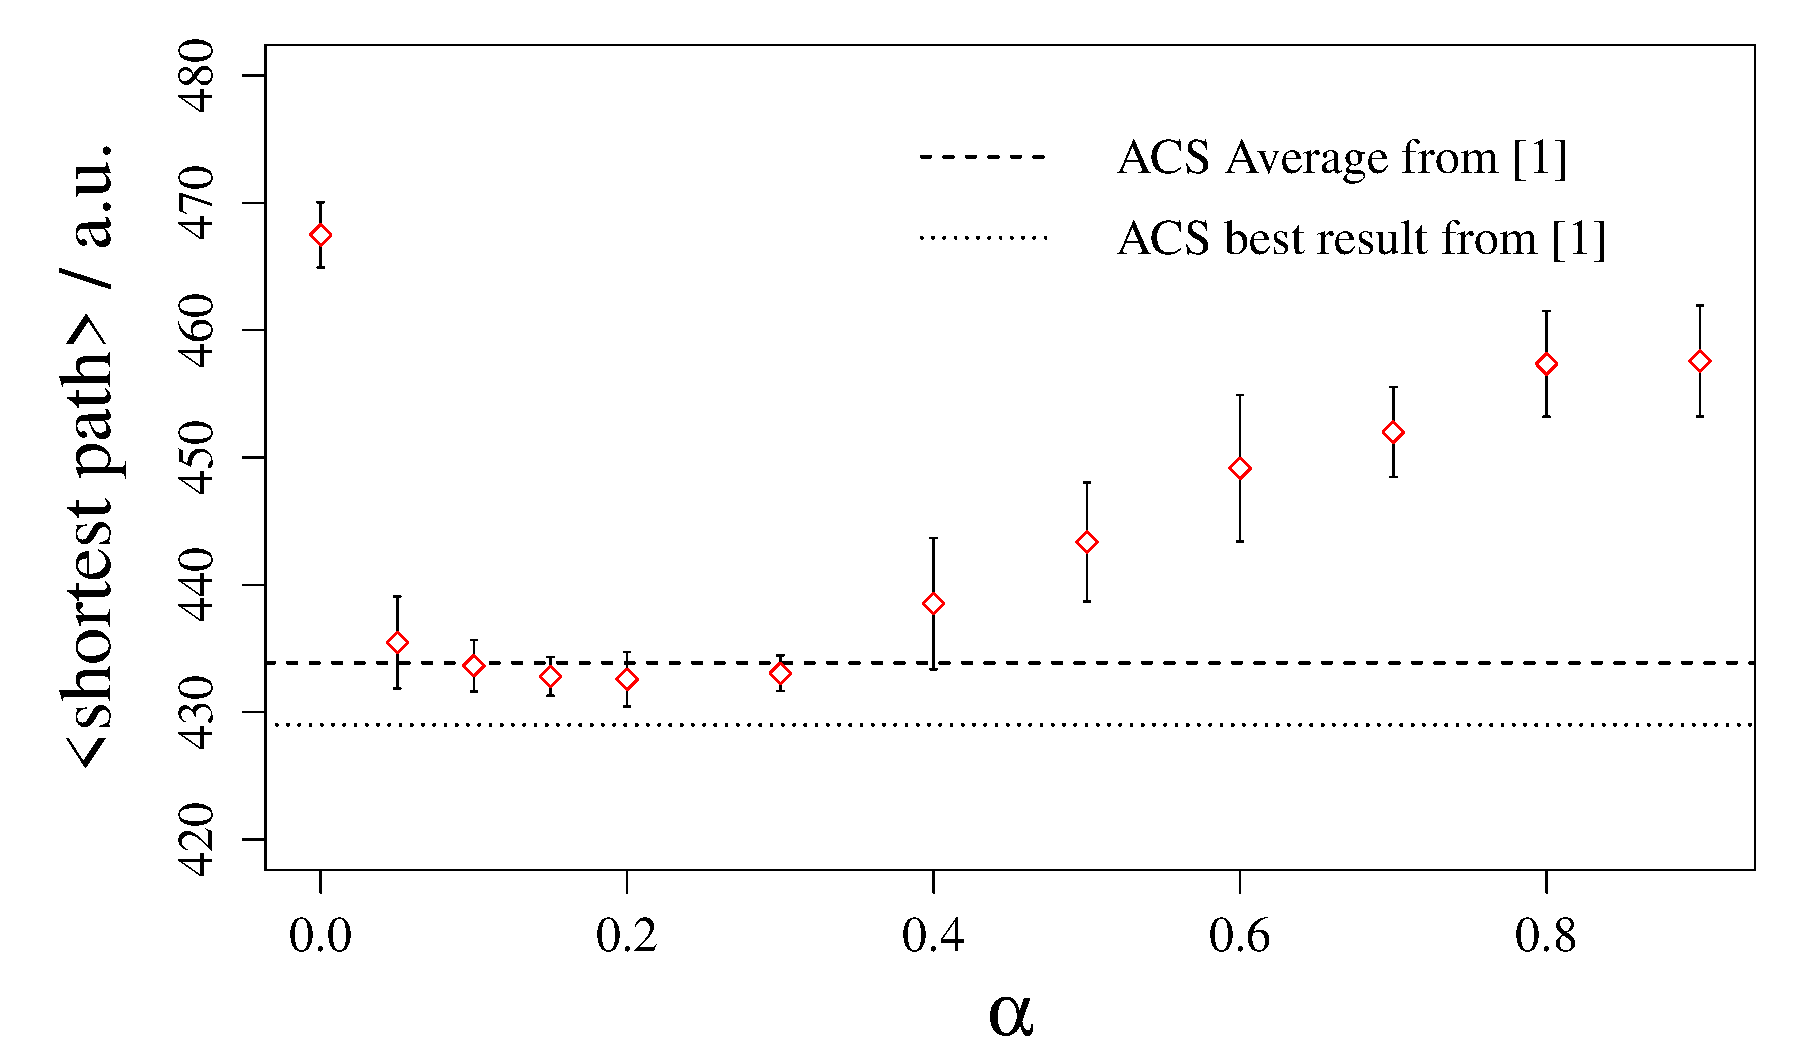
\includegraphics[width=11cm, height= 6 cm]{alpha_vs_shortestpath}
\caption{The update rate parameter $\alpha$ changes the averaged shortest tour length. The simulation is done for a fifty city problem using ten agents which all completed 2000 rounds. Other parameters are set to $beta=2$, $q_0=0.9$ and $tau_{\ref{start}}=0.1$. The values are averaged over ten runs. By setting $\alpha=0.1$ the length of the averaged shortest path is comparable to the value found in literature \cite{paper} and the change in pheromone update is held low.}
\label{fig:alphasp}
\end{center}
\end{figure}

For the parameter $\beta$ a similar analysis has been done for a thirty city environment and ten agents. The motivation for setting $\beta=2$ in \cite{paper} is barely understood from figure \ref{fig:betasp}. The decrease of the error for higher values of $\beta$ is explained by the fact that the criteria of closeness between the cities is weighted stronger than the pheromone concentration (see equation (\ref{eq:prob}) and (\ref{eq:qsmallerq0})). Thus, the exploration of new paths is suppressed and the deviation from the averaged path length is small. In the region of $\beta\approx2$ the bigger error bars indicate that the relative importance of pheromone and closeness is chosen such that the ants are forced to try new trails. The probability of getting stuck in a local minimum is reduced.

\begin{figure}[h!]
\begin{center}
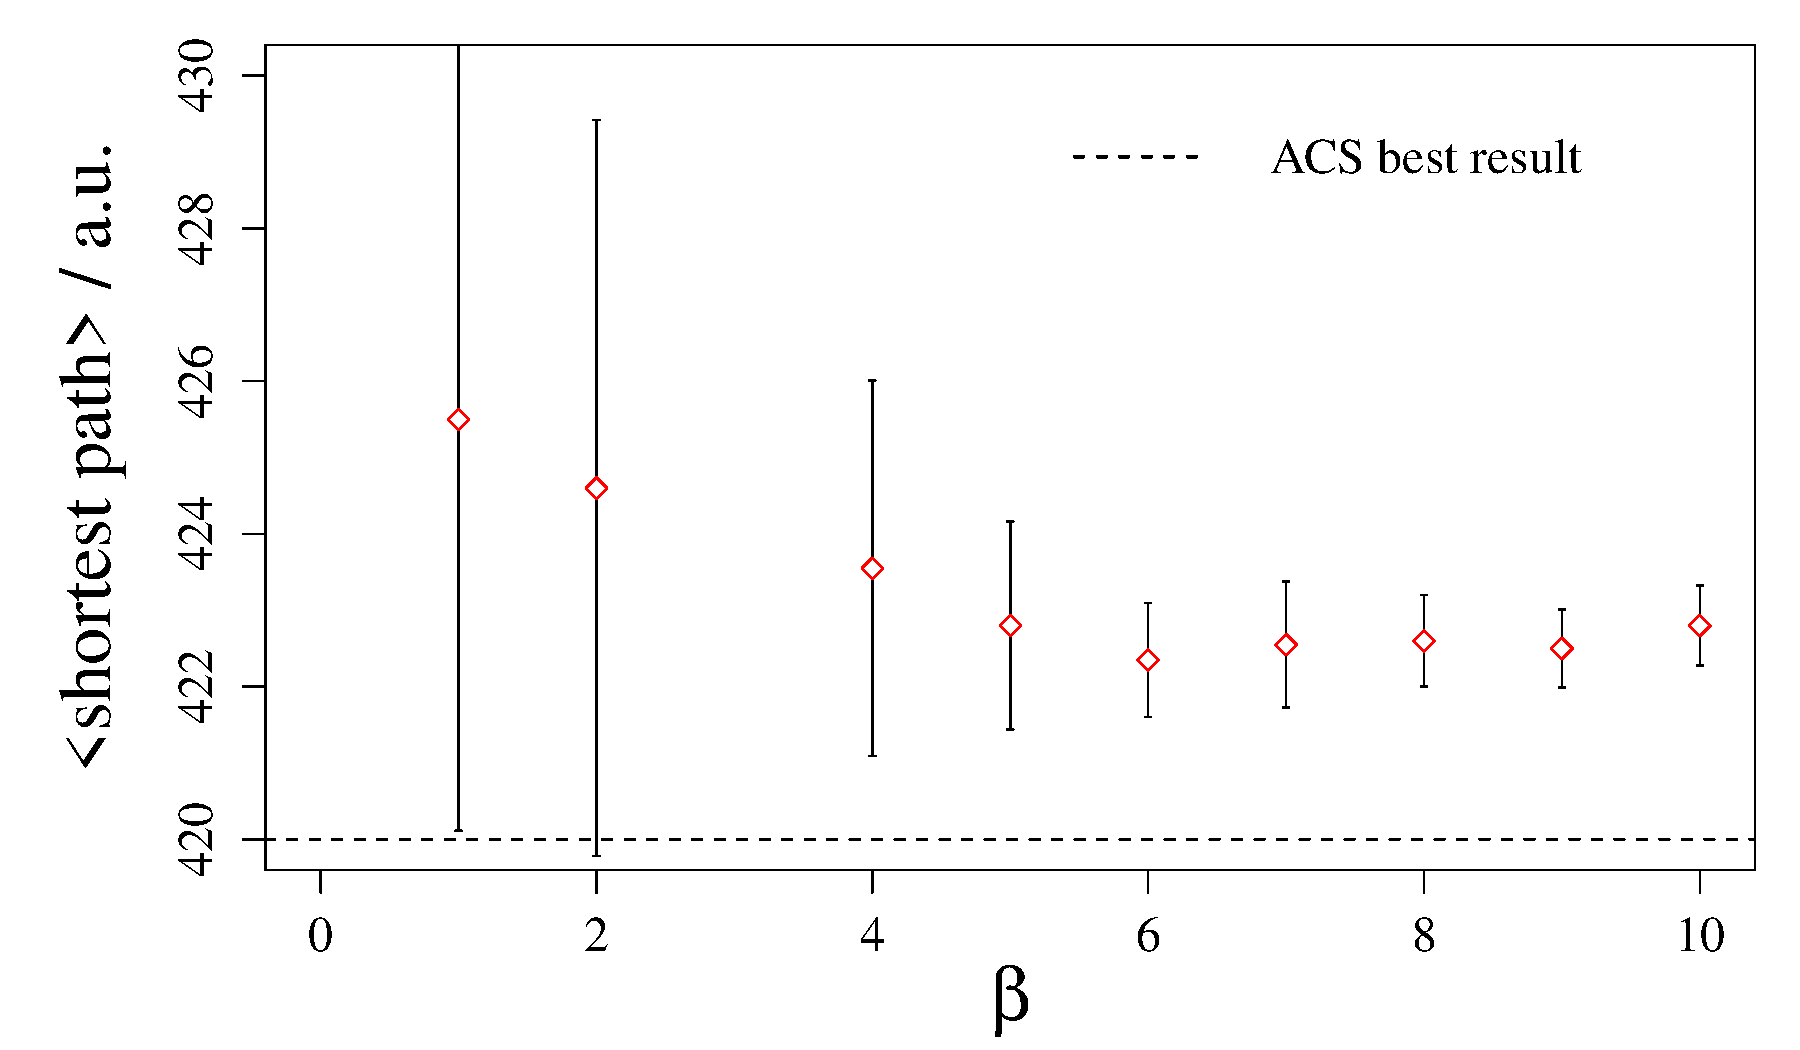
\includegraphics[width=11cm, height= 6 cm]{beta_vs_shortestpath}
\caption{Variation of the parameter $\beta$ for the oliver30 using ten ants going 400 rounds averaged over 20 runs. The parameters are chosen as $\alpha=0.1$,$q_0=0.9$ and $tau_{\ref{start}}=0.1$.}
\label{fig:betasp}
\end{center}
\end{figure}



\subsection{Model adaptions}



\section{Summary and Outlook}

\section{References}






\end{document}  



 
